In this chapter, we develop a Fortran90 \BoxLib\ code to solve the heat equation,
\begin{equation}
\frac{\partial\phi}{\partial t} = \nabla^2 \phi; \quad \phi(t=0) = e^{-100r^2},
\end{equation}
on a domain from -1 to 1 in each spatial direction, where $r$ is the distance
from the a cell-center to the center of the computational domain.  We will
assume that $\Delta x = \Delta y = \Delta z$.  We begin with a simple single-level, 
forward Euler discretization and work up to
a full AMR code with many bells and whistles.  Below is an outline of how we will 
proceed.  Each of these sections contains an accompanying tutoral directory.
\begin{itemize}

\item In Section \ref{Sec:OpenMP}, we develop a single-level code similar to the
previously discussed {\tt WaveEquation\_F} example, but add support for OpenMP.

\item In Section \ref{Sec:Boundary Conditions} we develop the capability to handle
other (non-periodic) boundary condition types.

\item In Section \ref{Sec:Refinement} we develop the capabilitly to have multiple
levels of refinement using a fixed, multilevel grid structure.

\item In Section \ref{Sec:AMR} we develop the capability to adaptively change the
refined grid structure.

\item In Section \ref{Sec:Linear Solvers} we develop the capability to solve the
equation implicitly, using the linear solver libraries.

\item In Section \ref{Sec:Checkpoints} we develop the capability to write and read
checkpoints for restarting simulations.

\end{itemize}
The basic time-advancement strategy uses the following temporal discretization:
\begin{equation}
\frac{\phi_{ij}^{n+1} - \phi_{ij}^n}{\Delta t} = \left[\nabla\cdot(\nabla\phi)\right]_{ij}.
\end{equation}
In the explicit case, we first compute $\nabla\phi$, at faces using:
\begin{equation}
(\nabla\phi)_{i+\myhalf,j} = \frac{\phi_{i+1,j}^n-\phi_{ij}^n}{\Delta x}.
\end{equation}
We will refer to these face-centered gradients as ``fluxes''.
Next, we compute the update by taking the divergence of these fluxes,
\begin{equation}
\left[\nabla\cdot(\nabla\phi)\right]_{ij} = \frac{(\nabla\phi)_{i+\myhalf,j}-(\nabla\phi)_{i-\myhalf,j}}{\Delta x} + \frac{(\nabla\phi)_{i,j+\myhalf}-(\nabla\phi)_{i,j-\myhalf}}{\Delta y}.
\end{equation}
We use a flux divergence formulation because it will enable a more natural 
extension to multiple levels of refinement, where we will be concerned with
conservation across levels.  Note that in this explicit case, if $\Delta x = \Delta y$, 
the Laplacian reduces to the standard five (seven) point stencil two (three) dimensions.  

\section{OpenMP}\label{Sec:OpenMP}

\section{Boundary Conditions}\label{Sec:Boundary Conditions}
In order to understand how to implement boundary conditions, we shall 
first describe the general principles behind working with boundary conditions.
Then, we will provide simple examples in the tutorial directory that can be 
adapted to other applications.

The basic idea is that every grid has knowledge of the
boundary condition type at the low and high side edge in each direction.
Common boundary condition types are {\tt INFLOW}, {\tt OUTFLOW}, {\tt SLIP\_WALL},
{\tt NO\_SLIP\_WALL}, and {\tt PERIODIC}.
There is also an {\tt INTERIOR} boundary condition type, which 
will be explained below.  There is typically an integer mapping, e.g., {\tt INFLOW}=1,
{\tt OUTFLOW=2}, etc.  Consider grid 1 in Figure \ref{fig:bc_example1}.  The
low-x boundary condition is {\tt INFLOW}, and the high-y boundary condition is
{\tt NO\_SLIP\_WALL}.  The high-x and low-y boundary conditions are {\tt INTERIOR}, which
means that the ghost cells share the same physical space as cells in the valid region of 
another grid.  Note that for grids 6, 7, 10, and 11, the boundary condition type for
every side is {\tt INTERIOR}.
%%%%%%%%%%%%%%%%%%%%%%%%%%%%%%%%%%%%%
\begin{figure}[tb]
\centering
\includegraphics[width=4in]{./AdvancedTopics/bc_example1}
\caption{\label{fig:bc_example1}Two-dimensional example with 16 - 4$^2$grids with
{\tt INFLOW}, {\tt OUTFLOW}, and {\tt NO\_SLIP\_WALL} boundary conditions.
The numbers refer to the grid number.}
\end{figure}
%%%%%%%%%%%%%%%%%%%%%%%%%%%%%%%%%%%%%

Figure \ref{fig:bc_example2} demonstrates a problem with periodicity.  In this case,
the low-x boundary condition for grid 1 is {\tt PERIODIC}.  Note there are some
similarities between {\tt PERIODIC} and {\tt INTERIOR} boundary conditions when
it comes to filling ghost cells.  In fact, one can think of {\tt PERIODIC} as just
a special type of {\tt INTERIOR} boundary condition.
In both of these cases, when filling ghost cells,
data from the valid region of another grid is copied into ghost cells of the neighboring 
grid.  For the other boundary conditions types, the user can write custom boundary 
conditions routines to fill ghost cells, which can involve setting ghost cell values 
directly, or extrapolating values from interior points using some stencil.
%%%%%%%%%%%%%%%%%%%%%%%%%%%%%%%%%%%%%
\begin{figure}[tb]
\centering
\includegraphics[width=4in]{./AdvancedTopics/bc_example2}
\caption{\label{fig:bc_example2}Two-dimensional example with 16 - 4$^2$grids with
{\tt PERIODIC} and {\tt NO\_SLIP\_WALL} boundary conditions.
The numbers refer to the grid number.}
\end{figure}
%%%%%%%%%%%%%%%%%%%%%%%%%%%%%%%%%%%%%

Now, consider an example with refined grids.  Figure \ref{fig:bc_example3}
contains three grids at the next level of refinement.  In this case, for grid 1,
all of the boundary condition types are {\tt INTERIOR}, even though the neighboring
valid region data is at a coarser level of refinement.  For grid 2, the low-y
boundary condition is {\tt NO\_SLIP\_WALL}, and the low-x, high-x, and hi-y
boundary condition types are {\tt INTERIOR}.
%%%%%%%%%%%%%%%%%%%%%%%%%%%%%%%%%%%%%
\begin{figure}[tb]
\centering
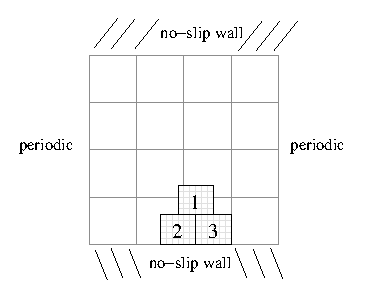
\includegraphics[width=4in]{./AdvancedTopics/bc_example3}
\caption{\label{fig:bc_example3}Two-dimensional example with 3 grids at a finer
resolution than the base grid.}
\end{figure}
%%%%%%%%%%%%%%%%%%%%%%%%%%%%%%%%%%%%%

\section{Multiple Levels of Refinement}\label{Sec:Refinement}
\section{Adaptive Mesh Refinement}\label{Sec:AMR}
\section{Linear Solvers}\label{Sec:Linear Solvers}
\section{Checkpoints and Restarting}\label{Sec:Checkpoints}


